\chapter{Experiments on Synthetic Graphs}

The methodology described is applied to two classes of synthetic networks. These generated benchmarks allow for the comparison to the ground truth communities, and also test how well each algorithm can extract networks in increasingly difficult problem spaces.

\section{Girvan-Newmann Experiments}
Here we present the results of each algorithm for a range of parameter sets on the Girvan-Newmann benchmark for a number of parameter sets for each of the selected algorithms.

Results are presented for $k_out$ values between 1 and 10, as after $k_out=8$ there is no strongly defined communities.


%%table            parameter set 1 | parameter set 2 | parameter set 3 | parameter set 4 | parameter set  5
% mixing parameter


%% convergence curves


\begin{figure}
	\begin{tabular}{cc}
		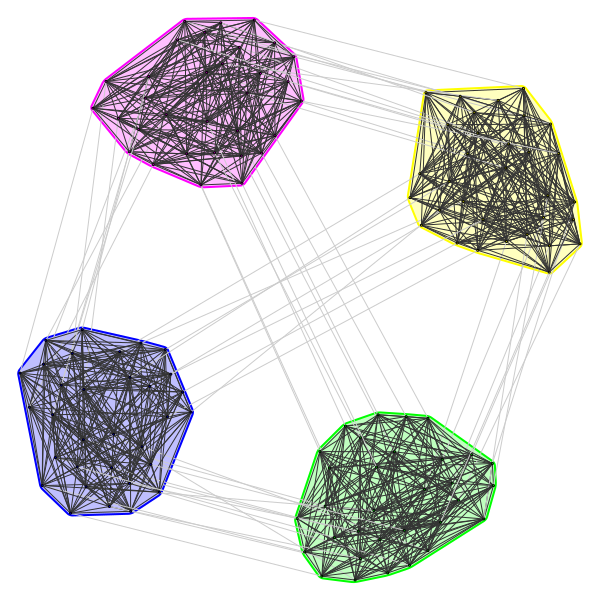
\includegraphics[width=65mm]{images/girvan_kout_1_0.png} &   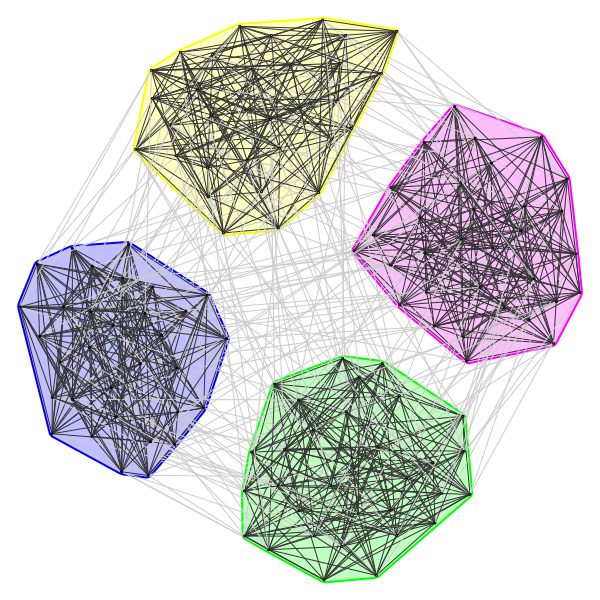
\includegraphics[width=65mm]{images/girvan_kout_3_0.png} \\
		(a) $k_{out}=1$ & (b) $k_{out}=3$ \\[6pt]
		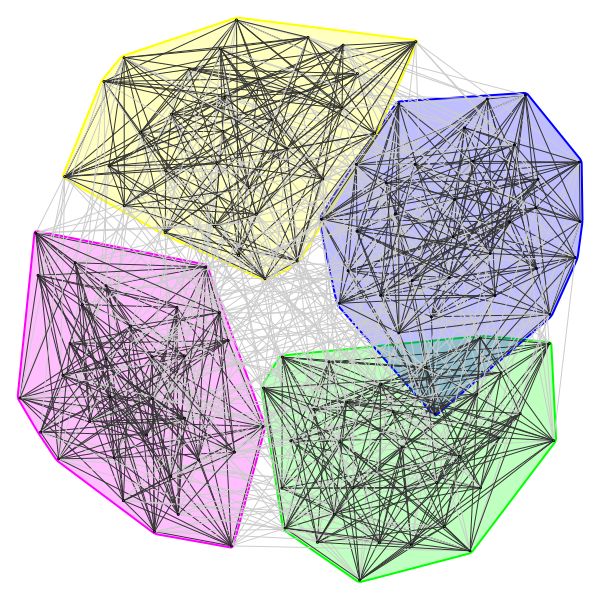
\includegraphics[width=65mm]{images/girvan_kout_5_0.png} &   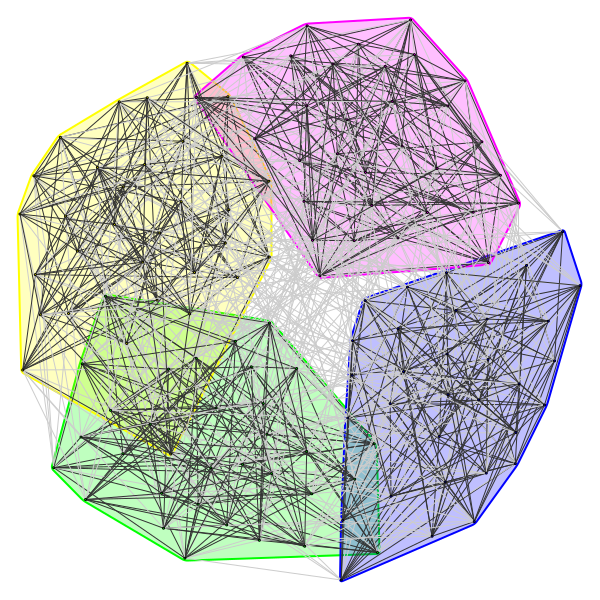
\includegraphics[width=65mm]{images/girvan_kout_6_0.png} \\
		(c) $k_{out}=5$ & (d) $k_{out}=6$ \\[6pt]
		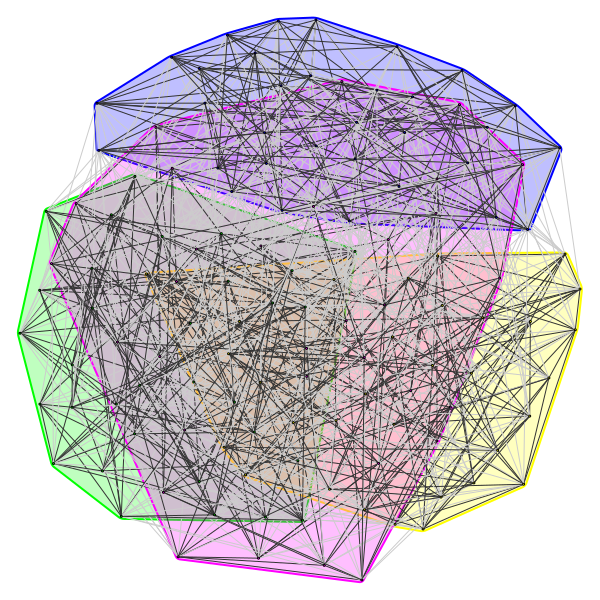
\includegraphics[width=65mm]{images/girvan_kout_8_0.png} &   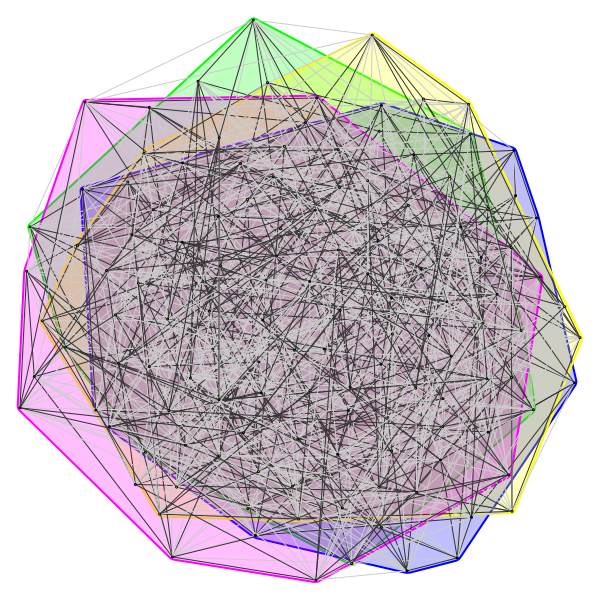
\includegraphics[width=65mm]{images/girvan_kout_10_0.png} \\
		(c) $k_{out}=8$ & (d) $k_{out}=10$ \\[6pt]
		
	\end{tabular}
	\caption{Visualizations of the GN benchmark with increasing $k_{out}$ parameters.}
\end{figure}


%% non-parametric tests

\section{LFR Benchmarks With Increasing Mixing \\ Parameter}
While the Girvan-Newmann benchmark allows for creating networks with increasingly difficult to identify communities, it is limited by its limits in terms of a fixed degree distribution, and no variance in community size. The LFR benchmark extends the planted $\ell$-partition model to allow a degree distribution following the power law and a mix of community sizes.

%%table            parameter set 1 | parameter set 2 | parameter set 3 | parameter set 4 | parameter set  5
% mixing parameter


%% lfr graph images


%% convergence curves

%% Extracted communities

%% non-parametric tests



\section{LFR Benchmarks With Increasing Size}
While an effective algorithm should detect communities even as the definition becomes more and more unclear from inter-community links, it should also be able to detect communities as the network scales in size. 
%% convergence curves

%% Extracted communities

%% non-parametric tests
